
\chapter{Introduction} \label{ch-1}

In recent years, a large amount of research addressing the contribution of intelligent
systems to cyber security has been conducted. One can hear more and more about artificial intelligence (AI), machine learning, and deep learning systems in cyber security.
As often happens with buzz words, nonexperts tend to use them casually and loosely.
Despite the fact that the borderlines between such terms are not always clear and these
borderlines become even fuzzier with new practical and theoretical developments, it is
important to try to characterize the focus of these systems in the field.


\section{AI: The next Frontier in IT Security} 

\textit{AI} in cybersecurity is a set of capabilities that allows organizations to detect, predict and respond to cyber threats in real-time
using machine and deep learning.


\textbf{AI-enabled cybersecurity is increasingly necessary}, organizations face an urgent need to continually ramp up and improve their cybersecurity. 

This is because the number of end user devices, networks and user interfaces continues to grow as a result of advances in cloud, the IoT,5G and conversational interfaces.

The increases the difficulty involved with administering a computer network. Having artificially intelligent network infrastructure that can learn to detect,
report and repair network security problems is an advantage to network administrators. 

Adaptability is another key reason that brought AI and computer security close to each other. The malicious entities that generate computer security attacks have gained intelligence. 
The type of attacks evolved from a simple password guessing to a staged and distributed network attack that can be equipped with a stealth mode and attack that mutation.
The compute security field has to adopt to rapid change and the evolution of security attacks. AI us well situated to answer this situation. AI is concerned with creating systems that evolve
and react depending on the changes in the surrounding environment. 

\textit{Fighting the Unknown}. For many years, the efforts of the IT security industry were based on the assumptions 
that attacks were conducted on a large scale and major threats spread before arriving at a specific network or computer.
Solutions were created on the basis of these assumptions and addressed as fellows. A typical threat was identified as a virus, which was investigated 
by IT security company labs that identified the virus signature and sent this information to endpoints installed with leading antivirus software. 

\textit{Internet of Things} In the past, most Internet interactions were interactions between humans that communicated via different platforms over the global network. 
Communications between humans, as the primary users of online communications will change dramatically with the evolution of the IoT realm ~\cite{Ko:2016:STU:2909066.2835492}. 

Most of the entities that will communicate on the Web in the future will be machines, and they will be used to initiate 
reports, make contact, or respond to requests. ~\cite{Komninos:2012}
The means to facilitate this is characterized by easy access to the Web and the ability for mass distribution. For example, there is a possibility to turn households into smart homes with 
intercommunicative technology instead of investing in designing a supporting infrastructure. 
Even scattering sensors along oil fields is the result of technological developments that led to a decrease in 
the price of materials, easy logistical operation, and resistant products that meet industrial standards. ~\cite{Chen:2017:DAI:3046067.3046227}

The cyber world has barely begun to focus on new types of dangers such as the autonomous world, since this process has just started. However, the severity 
level of the threat is clear. In coming years, the cyber defense community will be called upon to develop 
new and effective technologies to meet the challenges posed by our changing and increasingly autonomous world.


\section{The Contribution of Intelligent Systems to Cyber Security}\label{sec:cont-intelligent-systems-cyber-security}

Artificial intelligence (AI), which was officially established in the late 1950s by scholars such as Marvin Minsky, is used as a generic name representing a wide variety of
methods, tools, and techniques that mimic “cognitive” functions or tasks that people
associate with the human mind, such as “learning,” “planning,” “reasoning,” or “problem solving” ~\cite{Russell:1995}.
The importance of AI in cyber security is twofold and related to two opposing directions. The first direction focuses on 
AI-controlled systems as potential targets of cyber attacks, mainly due to their increasing role in controlling vital and complex 
systems. There are numerous examples of cyber risks related to AI-controlled systems, such as smart vehicles ~\cite{Berger:2013:PLC:2489103.2514809}
, smart grids and smart cities ~\cite{ALDAIRI20171086}.

\textbf{Knowledge-based systems and machine learning methods} are two well-known classes of AI methods that contain valuable tools
used in cyber security. In Knowledge-based systems, a huge amount of (experts') Knowledge is uploaded to the computer memory (thus, it is also called expert systems). ~\cite{Felgenbaum:1977:AAI:1622943.1623042}
The learning part in these systems is based on the reasoning related to this large body of knowledge, which is often obtained  by programmed rules (such as "if-then" and "inference logic rules").

Antivirus and antispam software packages ~\cite{Blanzieri:2008:SLT:1612711.1612715} represent straightforward
implementations of expert systems in cyber security. In this case, expert knowledge
(accumulated based on a large amount of transactions) regarding the procedures used—
such as applied protocols, network traffic (e.g., HTTP, HTTPS, VoIP, or email), and I/O
interactions with the operating system—is organized systematically to protect the
users from cyber breaches. There are several papers in this issue that serve as good
examples of such expert systems ~\cite{Maltinsky:2017:NNM:3055535.3040966} .


\textit{Machine-learning methods,} unlike knowledge-based systems, usually refer to applications in which the learning component is performed by the computers “themselves.”
This is often done by extracting relevant patterns from the data and using them to
derive predictions and smart recommendations. In other words, machine-learning algorithms are improved “automatically” through experience with the data, while giving
the computers “the ability to learn without being explicitly programmed,” as suggested
long before the field of cyber security was formally established ~\cite{Samuel:1959:SML:1661923.1661924}. There
are many examples of cyber-security tasks that can be addressed by machine learning,
including user monitoring, spam filtering, zero-day attack identification, risk analysis,
and many more.

It is well known that machine-learning methods are divided into two main classes
(and a hybrid class of methods that combines the two). The first class contains unsupervised learning methods, in which untagged data samples are introduced to the system
in order to find significant patterns. Fraud detection in financial systems, anomaly
detection in communication protocols, and segmentation of both users and software
packages according to their risk potential are good examples of unsupervised machine-
learning methods that apply techniques, such as anomaly detection and clustering, to
identify both “positive” or “negative” deviations from the norm. These deviations are
then mapped into actions that include, for example, risk assessment of new software
packages, blacklisted websites, or blocking Internet connections with high rates of suspicious users. Two papers published in this issue are introduced in this section, which
serve as good examples of unsupervised machine-learning methods ~\cite{Maltinsky:2017:NNM:3055535.3040966}
~\cite{Harel:2017:CSR:3055535.3057729}.

The second class of methods belongs to supervised learning, in which the data samples
that are introduced to the system are tagged a priori. In other words, the sample data
inputs are coupled with their desired outputs (thus the term supervised). The goal is to
learn a general rule that maps inputs to outputs. Some examples from the cyber security
domain are users’ risk scores ~\cite{Neria:2017:RFM:3055535.2928274}, for which descriptive features
of users—such as the communication volume, time, and the type of interaction—are
tagged either as “risky” or “nonrisky” and are then learned by the system to predict
high-risk users in advance ~\cite{Gruber:2018:UTB:3195275.3195331}.


Within the class of supervised-learning methods (that contain many other tools, such as decision trees, support vector machines, and regression models),
there is a unique group of artificial neural networks, which are models that were inspired by the structure and functional aspects of biological neural networks in the human brain.
Layers of nodes ("neurons") are connected to each other via weighted edges that are fine-tuned by mapping inputs
to tagged outputs.These models are often used to represent complex (nonlinear) relationships between inputs and outputs; 
they were considered to be very successful  and got another boost recently from the deep-learning revolution.

Deep learning models initially emerged from this subset of methods, consisting of neural
networks with multiple processing layers. These highly complex models require both
high-speed processing units and a large amount of data, which became more available
with the development of big-data technologies and cyber-security techniques. Deep-
learning models also evolved to address unsupervised learning and were found to be
extremely successful in signal processing (for which a lot of tagged data exists), specifically in image processing, which supports computer vision, and in speech recognition
~\cite{HeZRS16} ~\cite{hinton2012deep}, for which it has the primary task of identifying the
user and providing the user with the correct authorization level. These models gained
quite a bit of attention recently when leading global companies decided to invest 
significantly in these models in order to develop new applications; examples include Apple
(e.g., Siri), Alphabet/Google (e.g., self-driving cars), and Facebook (automated image
processing). These models have been shown to generate excellent results with specific
tasks, yet this performance is not always guaranteed, especially in noncontinuity cases
~\cite{Schmidhuber15}. Moreover, these models are not as descriptive as other analytic
models, such as closed-form regression models, decision trees, or graphical networks.
Therefore, their outputs pose challenges in terms of their interpretation or intuitive
understanding by cyber security analysts (that play a vital role in cyber defense)
~\cite{GanesanJC17} and by other decision makers (e.g., the Chief Information Officer)
in cyber security. Thus, deep learning is a subset of machine learning, which is a central
branch of AI. Deep learning should be viewed as an important tool in the cyber security
toolkit, specifically when the analytic tasks involved require modeling a large amount
of data by complex, often nonlinear, relations between the system’s input and output.

      To summarize, we believe that the role of intelligent systems in cyber security will
continue to grow, while the development of these systems, like any other scientific
development, poses both negative and positive effects on cyber security.


\section{Literature review} 

There have been several similar works done in IoT fields. Still, researchers are working in this area. Pahl et al. ~\cite{PahlA18} have
mainly developed a detector and firewall for an anomaly of IoT microservices in IoT site. 
Clustering methods like K-Means and BIRCH have been implemented ~\cite{AGGARWAL200381} for different microservices in this work. 
In clustering, different clusters were grouped in the same if the center is in the three times of standard deviation distance. 
The clustering model has been updated using an online learning technique. 
With the algorithms implemented, the overall accuracy obtained by the system is 96.3\%. 
A detailed description of a smart home system where security breaches were detected by deep learning method Dense
Random Neural Network (DRNN) ~\cite{BRUN2018458} have been introduced in ~\cite{BRUN2018458}.
They have mainly described Denial of Service attack and Denial of Sleep attack in a simple IoT site. 

Liu et al. ~\cite{LiuLLY18} proposed a detector for On and Off attack by a malicious network node in industrial IoT site. 
By On and Off attack they meant that IoT network could be attacked by a malicious node when it is in an active state or On state. 
Further- more, the IoT network behaves normal when its malicious node is in the inactive or off state. 
The system was developed using a light probe routing mechanism with the calculation of trust estimation of each neighbour node for the detection of an anomaly. 
Diro et al. ~\cite{DIRO2018761} discussed the detection of attack using fog-to-things architecture. 
The authors of the paper gave a comparison study of a deep and a shallow neural network using open source dataset. 
This work’s primary focus was to detect four classes of attack and anomaly. 
For four class the system got the accuracy of 98.27\% for deep neural network model and accuracy of 96.75\% for shallow neural network model. 
Usmonov et al. ~\cite{Usmonov8188589} described the recent security problem when developing embedded technologies for the IoT. 
Preserving data transfer between the physical, logical and virtual components of the IoT system was also challenging. 
For these problems, the use of digital watermarks was proposed by the authors of this work. 
Ukil et al. ~\cite{Ukil7474197} discussed the detection of anomalies in healthcare analytics based on IoT. 
A model of cardiac anomaly detection through a smartphone was also introduced in this paper. 
For the anomaly detection in healthcare; IoT sensors, medical image analysis, biomedical signal analysis, big data mining, and predictive analytics were used. 
Pajouh et al. ~\cite{Pajouh7762123} presented a model for intrusion detection based on a two-layer dimension reduction and two-tier classification module. 
This model was also designed to identify malicious activities such as User to Root (U2R) and Remote to Local (R2L) attacks. For dimension reduction, 
component analysis and linear discriminate analysis have been used. NSL-KDD dataset was used to carry out the whole experiment. 
For detecting suspicious behaviours with the two-tier classification module, Naive Bayes and Certainty Factor version of K-Nearest Neighbour were applied. 
D’Angelo et al. ~\cite{DANGELO2015408}  applied Uncertainty-managing Batch Relevance-based Artificial Intelligence (U-BRAIN) on binary NSL-KDD dataset and 
Real Traffic Data (from Fredrico II University of Napoli). The U-Brain is a dynamic model operated on multiple machines which can handle missing data. 
The NSL-KDD dataset contains 41 features. From 41 features 6 features.

\section{How organizations are benefiting from AI In cybersecurity}

\begin{itemize}
   \item {
      \textbf{AI lowers the cost to detect and respond to breaches:} Using AI for cybersecurity enables organizations to understand and reuse 
      threat patterns to identify new threats. This leads to an overall reduction in time and effort to identify incidents, investigate them, and remediate threats.
      Close to two-thirds of executives (64\%) say that AI lowers the cost to detect and respond to breaches. The reduction in cost for a majority of organizations ranges from 1\% – 15\% (with an average of 12\%). 
      However, a few organizations have managed to achieve even higher cost reductions (more than 15\%) leading to higher benefits (see \ref{fig-cost-to-detect-and-respond-to-breaches}).
      }
\end{itemize}

\begin{figure}[h]
   \center
   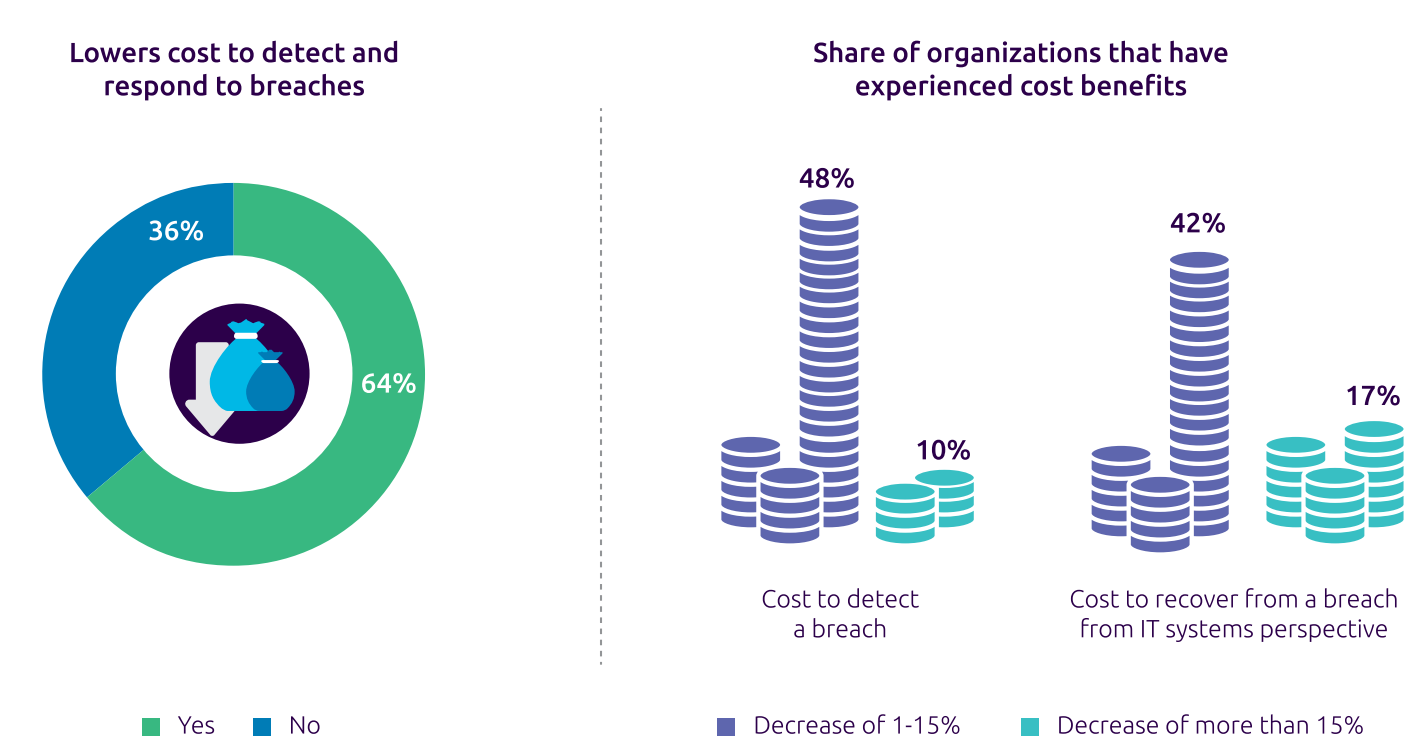
\includegraphics[width=.6\textwidth]{chap1/cost-to-detect-and-respond-to-breaches} 
   \caption{AI in cybersecurity lowers the cost to detect and respond to breaches ~\cite{Capgemini2019}.}
   \label{fig-cost-to-detect-and-respond-to-breaches}
\end{figure}

\begin{itemize}
   \item {
      \textbf{AI makes organizations faster at responding to breaches:}
      Fast response is essential to securing an organization from cyber attacks. With AI, the overall time taken to detect threats and breaches is reduced by up to 12\%. 
      AI also reduces the time taken to remediate a breach or implement patches in response to an attack by 12\%. A small subset of organizations even managed to reduce these time metrics by greater than 15\%
      zPower, a leading rechargeable battery manufacturer, partnered with a startup to use AI to detect and autonomously respond to threats as they emerge. Just weeks after the solution was deployed, 
      the security team was alerted to the fact that an employee had downloaded potentially malicious software. They were able to remove the threat and head off any attack in real time ~\cite{Darktrace2017}.
      (see ~\ref{fig-responding-to-breaches} \footnote{Source: Capgemini Research Institute, AI in Cybersecurity executive survey, $N$ $=$ $850$ executives})
      }
\end{itemize}

\begin{figure}[h]
   \center
   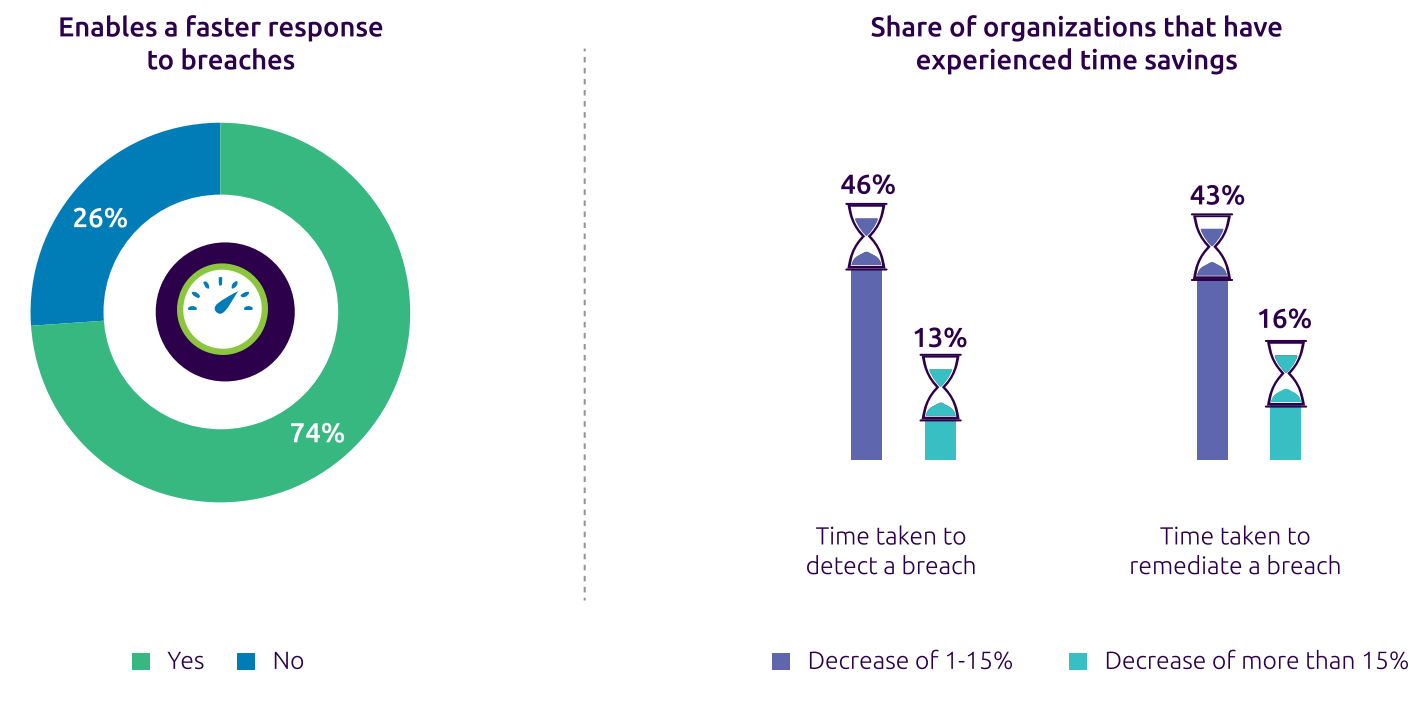
\includegraphics[width=.6\textwidth]{chap1/responding-to-breaches} 
   \caption{Nearly three in four executives say AI in cybersecurity enables a faster response to breaches
   Enables ~\cite{Capgemini2019}.}
   \label{fig-responding-to-breaches}
\end{figure}

\begin{itemize}
   \item {
      \textbf{AI results in higher efficiency for cyber analysts:} Cyber analysts spend considerable time going through data logs and/or incident timesheets. With AI helping carry that workload, cyber analysts can spend more quality time analyzing the incidents identified by the AI cybersecurity algorithms.
   }
\end{itemize}

\begin{figure}[ht]
   \center
   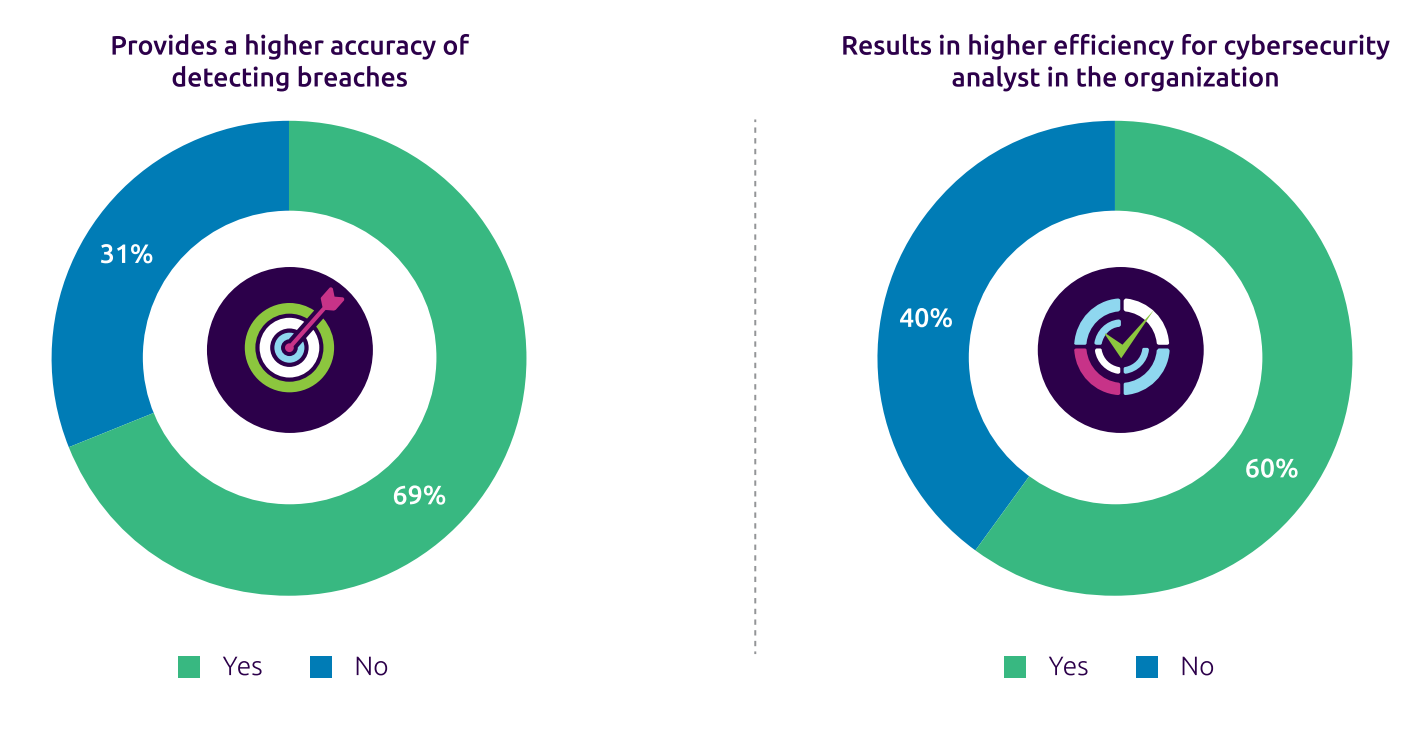
\includegraphics[width=.5\textwidth]{chap1/accuracy-of-detecting-breaches} 
   \caption{AI can help organizations provide a higher accuracy of detecting breaches
   Provides ~\cite{Capgemini2019}.}
   \label{fig-accuracy-of-detecting-breaches}
\end{figure}

\begin{itemize}
   \item {
      \textbf{AI results in new revenue streams through cybersecurity offerings:}
      With the proliferation of smart products – electronic devices generally connected wirelessly to other devices or networks – the attack surface for hackers increases. This creates an opportunity – offering cybersecurity services to manufacturers that sell smart products. A number of organizations are already targeting this opportunity:
          \begin{itemize}
             \item {
               \textbf{GE’s} Digital Ghost technology offers an AI-enabled protective layer for industrial control systems. Digital Ghost leverages the digital twins (which are often referred to as the brains of the associated control systems) to gain knowledge of the machine’s working pattern. Digital Ghost detects if the machine, while appearing to operate normally, 
               is actually being influenced by cyber attacks ~\cite{GEResearch2019}.
             }
             \item {
               Similarly, \textbf{Siemens’} ‘Industry Anomaly Detection’ solution uses AI to detect anomalies, either via intrusion or data theft by hackers. The solution analyzes data traffic in the network in a learning phase to establish transparency 
               of every device connected to the network. It can then identify any vulnerabilities while providing continuous monitoring to detect anomalies. ~\cite{Siemens20118}
             }
          \end{itemize}  
      }
\end{itemize}

\section{Research Plan}

 As an aims of the research and We provided a concrete plan for completion of the research including the design and 
 methods.

\begin{figure}[ht]
   \center
   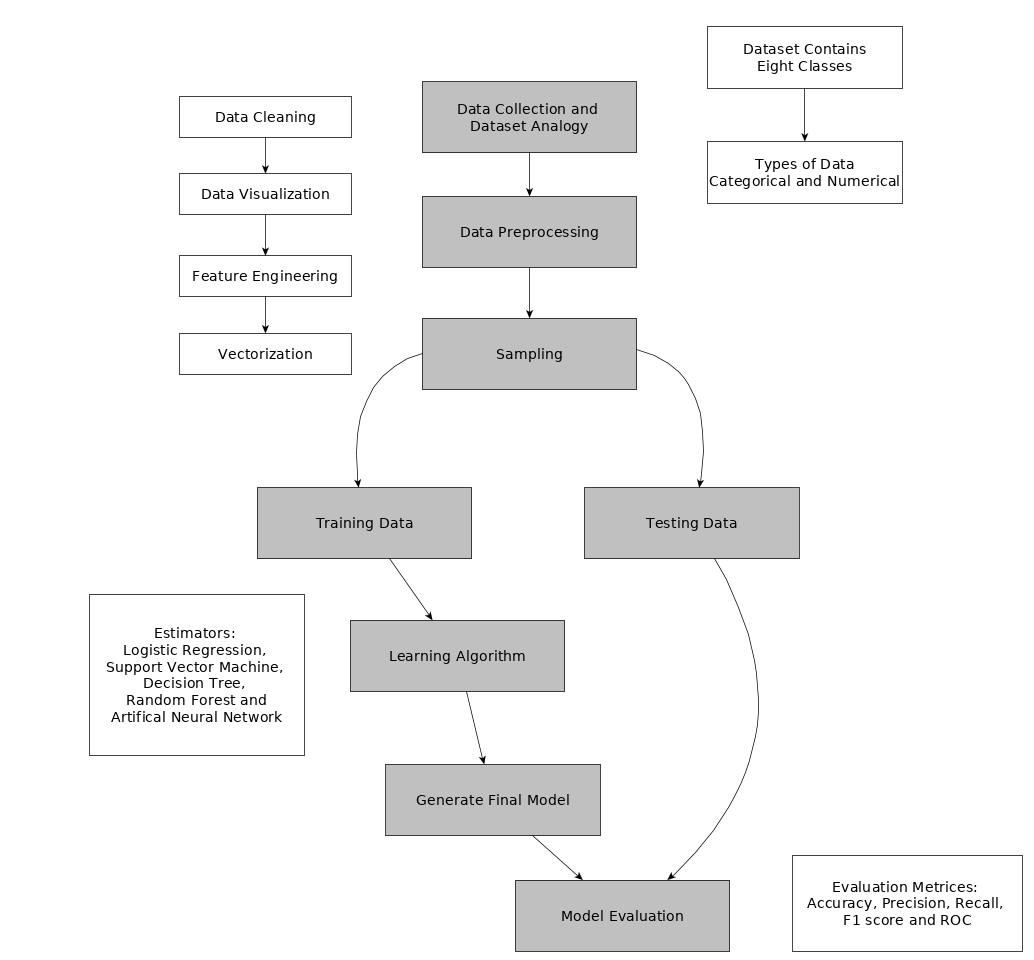
\includegraphics[width=.6\textwidth]{chap1/sec-framework-fig.png} 
   \caption{Overall framework for attack and anomaly detection in IoT and Cloud Base Services.}
   \label{fig-example}
\end{figure}

\begin{itemize}
   \item {
       Analyzing previous AI solutions which is developed for cybersecurity and figure out the deficiencies of the application. 
    }
   
    \item{
       Investigating "exploit databases" and collecting data related the kind of the threats.  
    }
    \item {
       Analyzing Cloud Based Systems' network infrastructures for collecting data. 
    }
   
    \item {
       Researching common and recent threats for the computer networks.
    }

    \item {
       Investigating the literature of the machine learning algorithms. 
   }
   \item {
       Analyzing the vulnerabilities of the cloud systems.   
   }

    \item {
       Defining the constraints of the problem.
    }

    \item {
       Modeling the problem. 
    }
    \item {
       Creating the fittest machine learning models for AI application 
    }
    \item {
       Developing the AI application that can detect, repair and defense the cloud based systems to against the cyber threats and attacks.
    }
   \item {
       Creating real-world test environment and creating real-time cyber-attacks scenarios for test the developed AI supported security applications.
   }

   \item {
       Regarding the test results of the application, optimize the AI algorithms with heuristic and metaheuristic approaches.  
   }

\end{itemize}